% ============================================================
%  CENG463 Final Project Report
%  Title : Epistemic Uncertainty in LLM Hallucinations
%  LNCS Template (Springer Lecture Notes in Computer Science)
%  Authors: Ata Türkyılmaz, Berkhan Kargılı, Atakan Kumbaracı
% ============================================================
\documentclass[runningheads]{llncs}

\usepackage[T1]{fontenc}
\usepackage[utf8]{inputenc}
\usepackage{graphicx}
\usepackage{booktabs}
\usepackage{amsmath,amssymb}
\usepackage{hyperref}
\usepackage{microtype}
\usepackage{multirow}
\usepackage{float}
\usepackage{subcaption}
\usepackage{url}

\hypersetup{colorlinks=true,linkcolor=black,citecolor=black,urlcolor=black}

% ============================================================
\begin{document}
% ============================================================

\title{Epistemic Uncertainty in LLM Hallucinations}

\titlerunning{Epistemic Uncertainty in LLM Hallucinations}

\author{Ata T\"{u}rky{\i}lmaz \and
        Berkhan Karg{\i}l{\i} \and
        Atakan Kumbarac{\i}}

\authorrunning{A. T\"{u}rky{\i}lmaz , B. Karg{\i}l{\i} , A. Kumbarac{\i}}

\institute{Department of Computer Engineering,
Izmir Institute of Technology, Izmir, Turkey\\
\email{\{ataturkyilmaz, berkhankargili, atakankumbaraci\}@std.iyte.edu.tr}\\
Repository: \url{https://github.com/TAtaTrkylmz/CENG463-FinalProject}}

\maketitle
\sloppy

% ============================================================
\begin{abstract}
Large language models (LLMs) remain prone to hallucination—generating fluent but factually incorrect outputs. A central hypothesis is that hallucinations coincide with elevated \emph{epistemic uncertainty}: when a model generates tokens outside its reliable knowledge, token-level probabilities become less confident. This paper presents a reproducible pipeline that investigates whether uncertainty signals from a low-cost local surrogate language model (\texttt{distilgpt2}) can classify hallucinated versus factual answers in the HaluEval QA benchmark. We implement ten complementary baseline detectors spanning four detection paradigms—lexical, uncertainty-based, semantic, and evidence/retrieval-grounded—alongside four hybrid models that combine these signal families, including a fine-tuned cross-encoder upper bound. An ablation study, structured error analysis, and two external evaluations complement the main benchmark. Results show the fine-tuned cross-encoder achieves the highest accuracy and macro F1 on the HaluEval validation split, while the Evidence-Aware Hybrid attains the highest AUROC; retrieval context yields measurable but modest gains over memory-only uncertainty features, suggesting token-level log-probability signals from a cheap surrogate are weak in isolation but complementary when combined with lexical or semantic cues. However, cross-dataset transfer is poor, and the Qwen-generated evaluation further suggests substantially weaker performance on actual generated answers, though this setting remains noisy due to prompt leakage and automatic labeling.
\end{abstract}

\keywords{Hallucination detection \and Epistemic uncertainty \and
          Large language models \and Token log-probabilities \and
          Retrieval-augmented generation \and HaluEval}

% ============================================================
\section{Introduction}
\label{sec:intro}
% ============================================================

Large language models (LLMs) remain prone to \emph{hallucination}: fluent but unsupported or false outputs~\cite{ji2023survey}. This matters most in high-stakes settings, where confidence and factuality can diverge sharply. In question answering, an answer may sound polished, specific, and locally coherent while still being factually wrong. As models become more capable, scalable, and conversational~\cite{brown2020gpt3,wei2022emergent}, this gap between fluency and truthfulness becomes harder for users to detect without external verification.

One natural hypothesis is that hallucinations correlate with elevated
\emph{epistemic uncertainty}. Following the standard distinction between
epistemic and aleatoric uncertainty~\cite{hullermeier2021aleatoric}, if a model is generating in regions where its
knowledge is weak or poorly grounded, token-level probabilities may become less
stable or less confident. This motivates the use of log-probability summaries,
entropy, and related white-box signals as potential hallucination indicators.
At the same time, modern models are also known to be overconfident~\cite{guo2017calibration},
so uncertainty is not guaranteed to track factuality cleanly. A useful detector
therefore needs to test not only whether uncertainty carries signal, but also
whether that signal remains useful once stronger semantic and evidence-based
features are available.

This problem sits between two different goals that are often conflated in the
literature. One goal is to build a practically robust hallucination detector
for arbitrary open-domain model outputs. The other is to understand, in a
controlled benchmark setting, which signal families are informative and how
they interact. Our project is explicitly closer to the second goal. We use
HaluEval QA~\cite{li2023halueval} as the main training and benchmarking
environment because it provides paired factual and hallucinated answers with a
shared question and knowledge snippet, making it suitable for comparative
analysis across multiple detectors. At the same time, earlier work on
faithfulness and factuality warns that hallucination is not a single failure
type: intrinsic and extrinsic errors can behave differently, and confidence can
degrade especially on long-tail knowledge or weakly grounded claims
~\cite{maynez2020faithfulness,mallen2023trust}.

We study this question with a fully reproducible local pipeline built around
\texttt{distilgpt2}~\cite{radford2019gpt2}. Our three research questions are:
\textbf{(RQ1)} whether cheap uncertainty features are predictive at all,
\textbf{(RQ2)} whether retrieved context improves them, and \textbf{(RQ3)}
whether uncertainty helps when fused with lexical, semantic, and evidence-based
signals. The main contribution is therefore not a claim of universal
hallucination detection, but a comparative benchmark: ten baselines, ablations,
structured error analysis, and transfer evaluation on both TruthfulQA-derived
pairs and Qwen-generated TruthfulQA answers. This framing matters because, as
our transfer results later show, strong in-domain performance may still fail to
generalise to open-domain generated outputs.

% ============================================================
\section{Related Work}
\label{sec:related}
% ============================================================

Prior work motivating this paper falls into three strands. The first is
\textbf{benchmarking hallucination itself}. HaluEval~\cite{li2023halueval}
provides paired factual and hallucinated responses across multiple tasks and is
well suited to controlled binary classification. TruthfulQA~\cite{lin2022truthfulqa}
takes a different angle: it targets questions that invite confident but false
answers, making it especially valuable for testing whether in-domain benchmark
gains survive transfer to harder open-domain settings. Together, these
benchmarks suggest that high apparent accuracy inside one dataset should not be
equated with general factual robustness. Related evaluation work such as
FActScore~\cite{min2023factscore} makes a similar point from another direction:
factual reliability is often better understood at the level of supported claims
than through surface plausibility alone.

The second strand is \textbf{uncertainty-based introspection}. Kadavath et
al.~\cite{kadavath2022know} show that language models can, to some degree,
reflect their own knowledge boundaries. Guo et al.~\cite{guo2017calibration}
show more broadly that modern neural models are often miscalibrated, which is
important because probability scores may still be informative even when they
are not perfectly trustworthy as absolute confidence estimates. Kuhn et
al.~\cite{kuhn2023semantic} further argue that naive token-level entropy can be
too brittle and propose \emph{semantic entropy}, which groups generations by
meaning before measuring uncertainty. We do not implement semantic entropy
here, but it serves as an important reference point for interpreting the limits
of small surrogate log-probability signals.

The third strand is \textbf{evidence-based grounding}. Retrieval-Augmented
Generation (RAG)~\cite{lewis2020rag} improves factuality by conditioning model
responses on external evidence, while SelfCheckGPT~\cite{manakul2023selfcheck}
uses agreement across multiple sampled outputs as a black-box reliability cue.
These approaches are relevant because they shift attention away from raw token
probabilities alone and toward whether an answer is supported by evidence or by
consistency across generations. Our NLI and context-comparison baselines are
inspired by this view.

Our contribution relative to this literature is narrower but practical: rather
than proposing a new frontier-scale detector, we compare uncertainty, lexical,
semantic, and evidence-based signals inside one local and reproducible pipeline.
That design lets us ask not only which method works best on HaluEval, but also
which families of signals degrade most severely once the evaluation moves to
TruthfulQA and actual model-generated answers.

% ============================================================
\section{Methodology}
\label{sec:method}
% ============================================================

The pipeline has four stages: dataset preparation, local LM scoring, baseline training, and hybrid-model training. All stages are orchestrated by \texttt{src/main.py}.

\subsection{Dataset and Problem Formulation}
\label{sec:data}

We use the QA split of HaluEval~\cite{li2023halueval}. Each record provides a question, a knowledge snippet, one factual answer, and one hallucinated answer. We expand each record into two supervised rows, factual ($y=0$) and hallucinated ($y=1$), producing balanced train/validation/test JSONL splits via \texttt{scripts/prepare\_dataset.py}. The main experiments use 15,999 training examples and 2,001 validation examples. This paired construction is useful for controlled comparison, but it may also introduce dataset-specific cues.

\subsection{Local Language Model Scoring}

Token-level log-probabilities are extracted with \texttt{distilgpt2}~\cite{radford2019gpt2}, used as a cheap local surrogate. For each candidate answer we compute mean log-probability, minimum log-probability, predictive entropy, and answer length. Scoring is done in both \emph{memory mode} (question + answer) and \emph{context mode} (knowledge prepended), allowing us to measure whether external evidence changes model confidence.

\subsection{Single-Signal Baselines}

We compare five single-signal baselines: a TF-IDF lexical SVM, two uncertainty classifiers (\texttt{entropy\_base} with \texttt{distilgpt2} and \texttt{entropy\_upgraded} with \texttt{Qwen/Qwen2.5-1.5B-Instruct}), a semantic SVM built from sentence-transformer interactions, a context-sensitive RAG comparison model based on the confidence shift $\Delta\bar{\ell}$, and an NLI evidence model using \texttt{roberta-large-mnli}. Together they represent shallow lexical cues, surrogate uncertainty, semantic compatibility, and evidence alignment.

\subsection{Hybrid and Joint Reasoning Models}

We also train four joint models: lexical and semantic hybrids that append uncertainty features to the corresponding base representations, an Evidence-Aware Hybrid that combines semantic, uncertainty, context-shift, and NLI signals, and a fine-tuned \texttt{distilroberta-base} cross-encoder as an upper-bound supervised baseline.

\subsection{Ablation Study Design}

Four ablations isolate feature-group contributions: \textit{lexical\_only}, \textit{uncertainty\_only}, \textit{hybrid\_no\_context}, and \textit{hybrid\_with\_context}.

% ============================================================
\section{Experiments}
\label{sec:experiments}
% ============================================================

\subsection{Setup}

The experiments use \texttt{Python~3.11}, \texttt{PyTorch~2.4},
\texttt{Transformers~4.44}, \texttt{scikit-learn~1.5}
\cite{pedregosa2011sklearn}, and dependencies pinned in
\texttt{requirements.txt}. The classification runs are fully local and
reproducible; some heavier generation and scoring steps can additionally use
GPU when available. Model weights are downloaded automatically via the Hugging
Face Hub. All randomness is controlled by fixed seeds. We report Accuracy,
Precision, Recall and macro-averaged F1 on the validation split. A random
baseline achieves 50\% accuracy on the balanced splits.

\subsection{Classification Results}

Table~\ref{tab:main_results} summarises performance across all ten methods. The Evidence-Aware Hybrid achieves the highest AUROC (0.9951), while the fine-tuned Cross-Encoder leads on Accuracy and Macro F1 (0.9815). Among single-signal baselines, the Semantic SVM is strongest; both entropy baselines trail the richer semantic and hybrid approaches.

\begin{table}[t]
  \centering
  \caption{Comprehensive hallucination detection results on the HaluEval QA
           validation split. Best results per metric are in bold.}
  \label{tab:main_results}
  \renewcommand{\arraystretch}{1.1}
  \begin{tabular}{llccc}
    \toprule
    & \textbf{Method} & \textbf{Acc.} & \textbf{Macro F1} & \textbf{AUROC} \\
    \midrule
    \multirow{6}{*}{\rotatebox{90}{Single-Signal}}
    & Lexical SVM           & 0.9381 & 0.9380 & 0.9729 \\
    & Entropy Base          & 0.9426 & 0.9425 & 0.9765 \\
    & Entropy Upgraded      & 0.9231 & 0.9231 & 0.9654 \\
    & Semantic SVM          & 0.9695 & 0.9695 & 0.9870 \\
    & NLI Evidence          & 0.7877 & 0.7866 & 0.7943 \\
    & RAG Compare Fixed     & 0.7522 & 0.7490 & 0.7723 \\
    \midrule
    \multirow{4}{*}{\rotatebox{90}{Hybrid}}
    & Lexical Hybrid SVM    & 0.9530 & 0.9530 & 0.9805 \\
    & Semantic Hybrid SVM   & 0.9675 & 0.9675 & 0.9878 \\
    & Evidence-Aware Hybrid & 0.9770 & 0.9770 & \textbf{0.9951} \\
    & Cross-Encoder (FT)    & \textbf{0.9815} & \textbf{0.9815} & 0.9895 \\
    \bottomrule
  \end{tabular}
\end{table}

\subsection{Ablation Results}

Table~\ref{tab:ablation} reports the ablation study for the lexical-uncertainty model family on the HaluEval QA validation split. Lexical features already provide a strong baseline (Macro F1 = 0.9390). Uncertainty features alone are substantially weaker under the default threshold (Macro F1 = 0.7152), although their AUROC remains high (0.9740), indicating useful ranking signal even in isolation. Adding the context-delta features produces the strongest ablation result overall, directly supporting RQ2.

\begin{table}[t]
  \centering
  \caption{Ablation study: marginal contribution of each feature group on the HaluEval QA validation split (linear SVM classifier, $n=2{,}002$ validation rows).}
  \label{tab:ablation}
  \renewcommand{\arraystretch}{1.1}
  \begin{tabular}{llccc}
    \toprule
    \textbf{Setting} & \textbf{Features} & \textbf{Acc.} & \textbf{Macro F1} & \textbf{AUROC} \\
    \midrule
    lexical\_only         & TF-IDF                                  & 0.9391 & 0.9390 & 0.9703 \\
    uncertainty\_only     & Log-probability features                & 0.7338 & 0.7152 & 0.9740 \\
    hybrid\_no\_context   & TF-IDF + log-probability features       & 0.9446 & 0.9446 & 0.9800 \\
    hybrid\_with\_context & TF-IDF + log-probability + $\Delta$     & \textbf{0.9735} & \textbf{0.9735} & \textbf{0.9919} \\
    \bottomrule
  \end{tabular}
\end{table}

\subsection{Transfer Evaluation}

To test external validity, we evaluated the HaluEval-trained detectors on two
out-of-domain settings: a TruthfulQA-derived binary evaluation set (1,634 rows)
and a harder set of 817 \texttt{Qwen/Qwen2.5-1.5B-Instruct} generations from
TruthfulQA questions. Table~\ref{tab:transfer_summary} shows the main pattern.
High HaluEval accuracy does not transfer reliably. The Cross-Encoder drops from
0.9815 to 0.5477 on TruthfulQA pairs and 0.4712 on Qwen-generated answers; the
Semantic SVM drops from 0.9695 to 0.5208 and 0.4749; the Entropy Base model
falls from 0.9426 to 0.5024 and 0.4847. Evidence-grounded methods transfer
better on benchmark-written TruthfulQA answers, especially NLI Evidence
(0.9694 Accuracy, 0.9943 AUROC), but they also weaken sharply on the
Qwen-generated set. We interpret that second result more cautiously than the
canonical TruthfulQA transfer table, because a post-hoc audit revealed prompt
leakage and weak automatic NLI labels in part of the generated evaluation set.
Even with that caveat, the main qualitative pattern remains useful: the
pipeline is no longer evaluated only inside HaluEval, and the transfer gap is
explicit rather than assumed.

\begin{table}[t]
  \centering
  \caption{Transfer performance from HaluEval QA training to two out-of-domain evaluation sets.}
  \label{tab:transfer_summary}
  \renewcommand{\arraystretch}{1.08}
  \small
  \begin{tabular}{lccccc}
    \toprule
    \textbf{Method} & \textbf{HaluEval} & \textbf{TruthfulQA} & \textbf{TQA AUROC} & \textbf{Qwen-Gen} & \textbf{QG AUROC} \\
    \midrule
    Cross-Encoder    & 0.9815 & 0.5477 & 0.5764 & 0.4712 & 0.4924 \\
    Entropy Base     & 0.9426 & 0.5024 & 0.4863 & 0.4847 & 0.5062 \\
    Semantic SVM     & 0.9695 & 0.5208 & 0.4750 & 0.4749 & 0.4344 \\
    Evidence-Aware   & 0.9770 & 0.5967 & 0.8665 & 0.4847 & 0.4832 \\
    NLI Evidence     & 0.7877 & 0.9694 & 0.9943 & 0.5129 & 0.7034 \\
    RAG Compare      & 0.7522 & 0.8635 & 0.9514 & 0.4847 & 0.5506 \\
    \bottomrule
  \end{tabular}
\end{table}

% ============================================================
\section{Error Analysis}
\label{sec:error}
% ============================================================

We analyse errors by answer length and decision-margin confidence because raw
aggregate metrics hide distinct failure modes. Figure~\ref{fig:combined_errors}
shows that lexical, uncertainty, semantic, and evidence-based systems break
down under different conditions even when their headline scores are all high.

\textbf{Short answers are the hardest subgroup.} Across nearly all baselines,
error rates peak in the shortest answer bucket and drop as answers become
longer. This is intuitive once we inspect the feature families. Short responses
contain fewer informative n-grams, fewer tokens over which log-probability
statistics can stabilize, and less semantic structure for interaction models to
use. Many HaluEval hallucinations are also short and stylistically plausible,
so they can look like normal factual answers unless the model has access to a
strong evidence signal. This is consistent with the broader phenomenon of
high-confidence hallucination, where wrong answers can remain locally fluent and
confident despite being factually unsupported~\cite{zhang2023highcert}. In this
regime, even small wording choices can dominate the decision boundary.

This finding turns a reviewer criticism into a concrete modeling diagnosis. We
tested a length-aware extension of the Evidence-Aware Hybrid using
separate short/long experts with a 40-token threshold. However, it did not
improve results (Accuracy 0.9770 $\rightarrow$ 0.9760; AUROC 0.9951
$\rightarrow$ 0.9950). The likely reason is that HaluEval is overwhelmingly
short-form under this definition, so the split does not create two genuinely
different learning regimes. In other words, the weakness is real, but a naive
bucketed solution is not enough. Better short-answer handling will likely
require stronger entity matching, tighter evidence comparison, or calibration
strategies designed specifically for brief and underspecified claims.

\textbf{Evidence-only signals are more overconfident.} The confidence
stratification also reveals an important contrast between model families.
Lexical and semantic models concentrate most of their errors in the lowest
confidence region; once they become even moderately confident, their error rates
fall quickly. By contrast, evidence-comparison baselines such as RAG Compare
and, to a lesser extent, NLI Evidence retain noticeable errors even at higher
decision margins. This suggests that the raw confidence shift caused by adding
context is not a clean factuality score by itself. A large or small
$\Delta\bar{\ell}$ may reflect stylistic compatibility with the added context,
surface overlap, or quirks of the surrogate language model rather than true
grounding.

\textbf{Hybrid models fail more gracefully.} The best joint systems reduce
exactly these brittle behaviors. The Evidence-Aware
Hybrid combines semantic interaction, NLI support, and uncertainty summaries,
and its error profile is much flatter in the high-confidence region than the
evidence-only baselines. This supports the broader interpretation of the paper:
uncertainty and evidence signals are useful, but they are strongest when they
act as complementary constraints rather than as standalone decision rules. The
error analysis therefore reinforces the main quantitative results. The problem
is not that uncertainty is useless; it is that isolated uncertainty and
isolated evidence shifts remain too fragile on the most ambiguous, short, and
plausible answers.

\begin{figure}[H]
  \centering
  \begin{subfigure}[b]{0.49\textwidth}
    \centering
    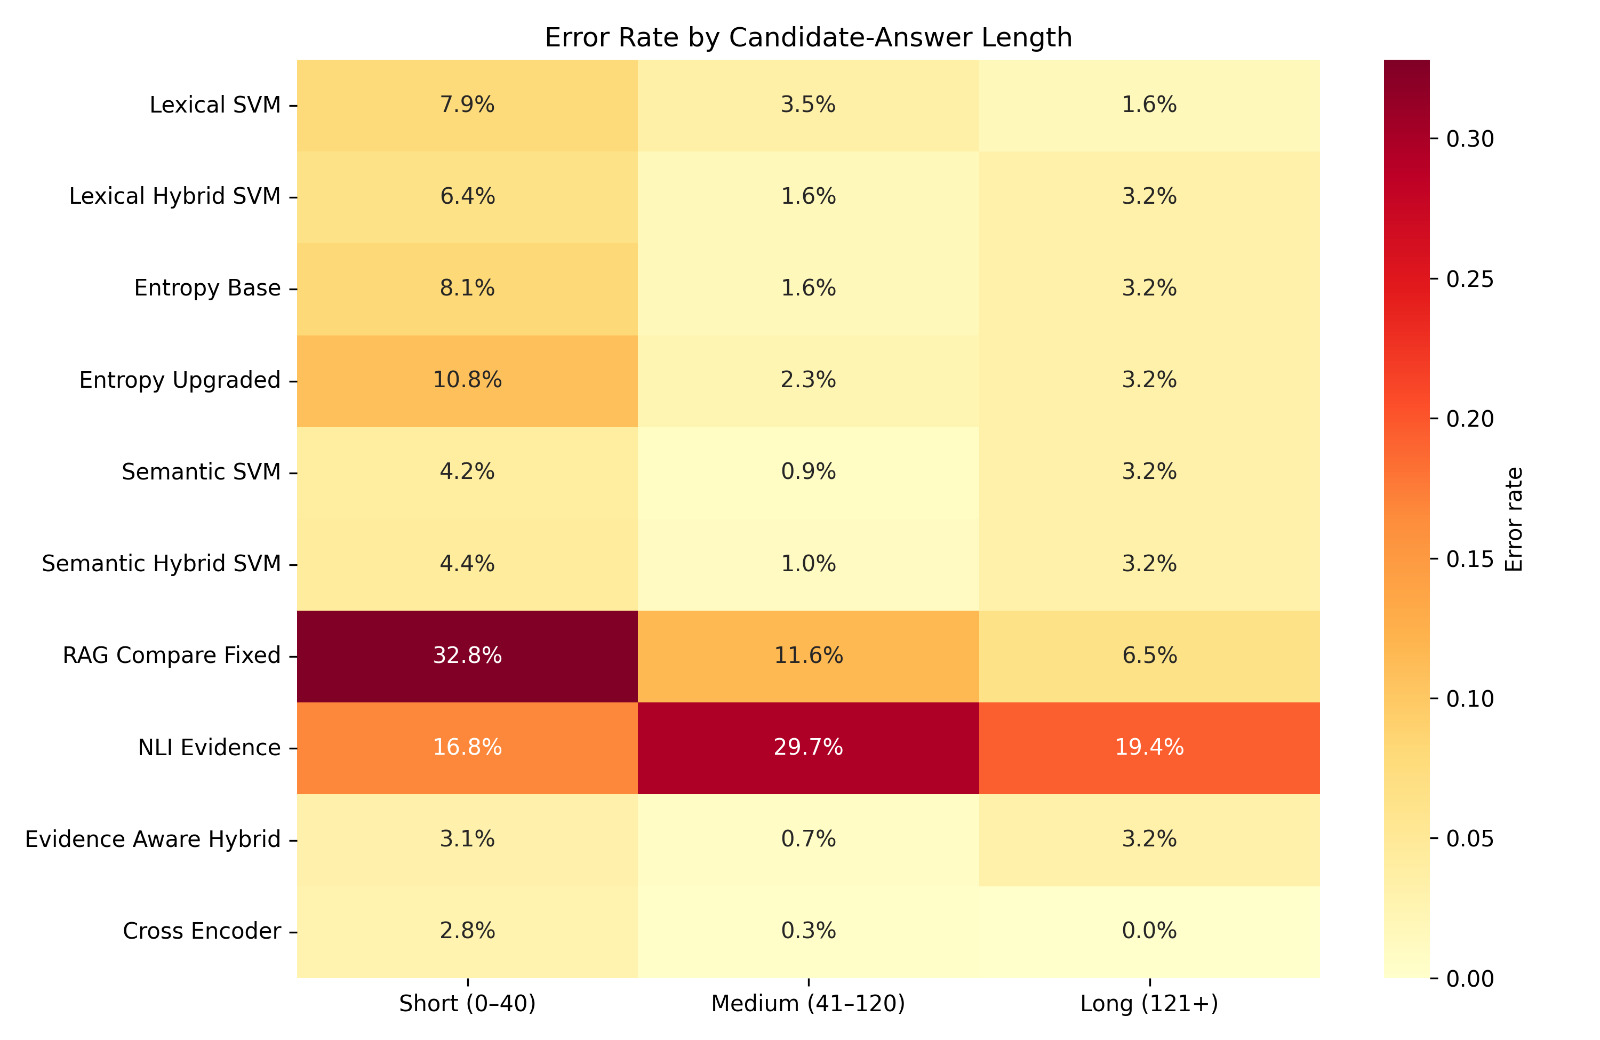
\includegraphics[width=\textwidth]{fig_error_length}
    \caption{Stratification by answer length.}
    \label{fig:error_length}
  \end{subfigure}
  \hfill
  \begin{subfigure}[b]{0.49\textwidth}
    \centering
    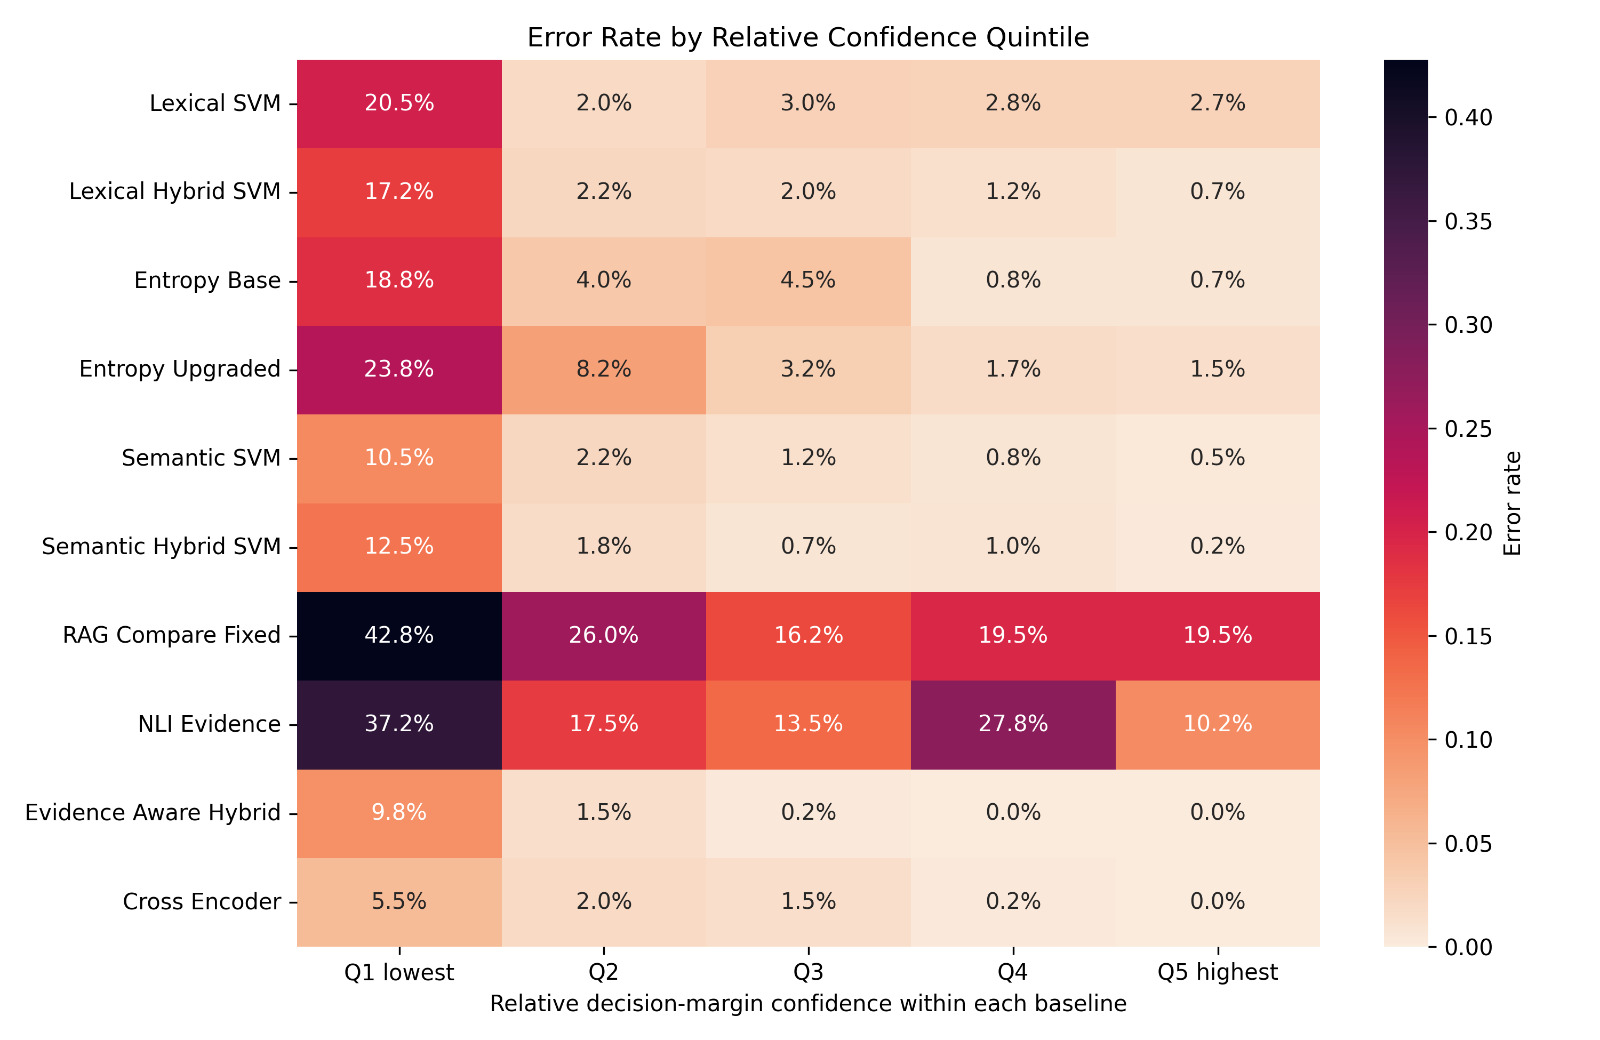
\includegraphics[width=\textwidth]{fig_error_confidence}
    \caption{Stratification by confidence.}
    \label{fig:error_confidence}
  \end{subfigure}
  \caption{Error rate analyses across baseline models.}
  \label{fig:combined_errors}
\end{figure}

% ============================================================
\section{Conclusion}
\label{sec:conclusion}
% ============================================================
\raggedbottom

\textbf{Interpretation.} Our results support a narrower claim than a generic
``hallucination detector'' story. Token-level log-probability features from
\texttt{distilgpt2} carry real signal, but they are not the strongest standalone
family and work best when combined with semantic or evidence-aware features.
Replacing \texttt{distilgpt2} with \texttt{Qwen2.5-1.5B-Instruct} did not help:
the upgraded entropy baseline drops from 0.9425 to 0.9231 Macro F1, suggesting
that stronger next-token modeling does not automatically yield a more useful
factuality signal. The ablation and hybrid results point to the same practical
lesson: uncertainty is complementary, not sufficient, and the change in model
confidence after adding evidence is more informative than raw confidence alone.

\textbf{Limitations and Future Work.} The main limitation remains external
validity. Although we now evaluate on both TruthfulQA-derived pairs and
Qwen-generated TruthfulQA answers, all supervised training is still done on
HaluEval QA, whose paired construction can reward dataset-specific artifacts.
The uncertainty signal is also taken from a surrogate model rather than from
the original generator, so it should be interpreted as a cheap proxy rather
than a direct measure of the source model's epistemic state. In addition, the
Qwen-generated TruthfulQA evaluation set was labeled automatically using NLI,
and our audit found noticeable prompt leakage and many low-margin label
decisions; that generated-output experiment is therefore best read as
indicative rather than fully clean ground truth. Short answers also remain a
genuine weakness: we tested a simple length-aware expert split, but it did not
improve results because HaluEval is overwhelmingly short-form. The next step is
therefore not merely ``add a length feature,'' but to move toward stronger
uncertainty families such as semantic entropy~\cite{kuhn2023semantic} or
self-consistency, train or calibrate on more realistic open-domain
generations, and design short-answer handling that relies more on entity and
evidence matching than on coarse length buckets.

\textbf{Conclusion.} We presented a reproducible pipeline for comparing
uncertainty, semantic, and evidence-based hallucination detectors on HaluEval
QA. Within the benchmark, hybrid and cross-attentive models perform extremely
well. Outside it, however, performance drops sharply, and the Qwen-generated
evaluation further suggests that real model outputs are harder than
benchmark-written answers, even though that generated set still contains label
noise and prompt artifacts. The main contribution of the project is therefore
methodological and diagnostic: it shows where cheap uncertainty signals help,
where they fail, and why open-domain hallucination detection still requires
stronger generation-aware and evidence-aware modeling.

\pagebreak
% ============================================================
\begin{thebibliography}{99}

\bibitem{ji2023survey}
Ji, Z. et al.:
Survey of hallucination in natural language generation.
ACM Comput.\ Surv.\ \textbf{55}(12), 1--38 (2023).
\href{https://doi.org/10.1145/3571730}{doi:10.1145/3571730}

\bibitem{li2023halueval}
Li, J., Cheng, X., Zhao, W.X., Nie, J.-Y., Wen, J.-R.:
HaluEval: A large-scale hallucination evaluation benchmark for large language models.
In: Proc.\ EMNLP 2023, pp.~6449--6464. ACL, Singapore (2023).
\href{https://doi.org/10.18653/v1/2023.emnlp-main.397}{doi:10.18653/v1/2023.emnlp-main.397}

\bibitem{hullermeier2021aleatoric}
H\"{u}llermeier, E., Waegeman, W.:
Aleatoric and epistemic uncertainty in machine learning: An introduction to concepts and methods.
Mach.\ Learn.\ \textbf{110}(3), 457--506 (2021).
\href{https://doi.org/10.1007/s10994-021-05946-3}{doi:10.1007/s10994-021-05946-3}

\bibitem{kadavath2022know}
Kadavath, S. et al.:
Language models (mostly) know what they know.
arXiv:2207.05221 (2022).
\href{https://arxiv.org/abs/2207.05221}{arXiv:2207.05221}

\bibitem{kuhn2023semantic}
Kuhn, L., Gal, Y., Farquhar, S.:
Semantic uncertainty: Linguistic invariances for uncertainty estimation in natural language generation.
In: Proc.\ ICLR 2023. OpenReview (2023).
\href{https://openreview.net/forum?id=VD-AYtP0dve}{openreview.net/forum?id=VD-AYtP0dve}

\bibitem{lewis2020rag}
Lewis, P. et al.:
Retrieval-augmented generation for knowledge-intensive NLP tasks.
In: Proc.\ NeurIPS 2020, vol.~33, pp.~9459--9474 (2020).

\bibitem{manakul2023selfcheck}
Manakul, P., Liusie, A., Gales, M.J.F.:
SelfCheckGPT: Zero-resource black-box hallucination detection for generative large language models.
In: Proc.\ EMNLP 2023, pp.~9004--9017. ACL, Singapore (2023).
\href{https://doi.org/10.18653/v1/2023.emnlp-main.557}{doi:10.18653/v1/2023.emnlp-main.557}

\bibitem{radford2019gpt2}
Radford, A., Wu, J., Child, R., Luan, D., Amodei, D., Sutskever, I.: Language models are unsupervised multitask learners.
OpenAI Blog \textbf{1}(8), 9 (2019).

\bibitem{guo2017calibration}
Guo, C., Pleiss, G., Sun, Y., Weinberger, K.Q.: On calibration of modern neural networks.
In: Proc.\ ICML 2017, PMLR vol.~70, pp.~1321--1330 (2017).
\href{https://proceedings.mlr.press/v70/guo17a.html}{proceedings.mlr.press/v70/guo17a.html}

\bibitem{pedregosa2011sklearn}
Pedregosa, F. et al.:
Scikit-learn: Machine learning in Python.
J.\ Mach.\ Learn.\ Res.\ \textbf{12}, 2825--2830 (2011).
\href{https://jmlr.org/papers/v12/pedregosa11a.html}{jmlr.org/papers/v12/pedregosa11a.html}

\bibitem{zhang2023highcert}
Simhi, A., Markovitch, S.:
Trust me, I'm wrong: LLMs hallucinate with certainty despite knowing the answer.
arXiv:2502.12964 (2025).
\href{https://arxiv.org/abs/2502.12964}{arXiv:2502.12964}

\bibitem{brown2020gpt3}
Brown, T. et al.:
Language models are few-shot learners.
In: Proc.\ NeurIPS 2020, vol.~33, pp.~1877--1901 (2020).

\bibitem{wei2022emergent}
Wei, J. et al.:
Emergent abilities of large language models.
Trans.\ Mach.\ Learn.\ Res.\ (2022).
\href{https://openreview.net/forum?id=yzkSU5zdwD}{openreview.net/forum?id=yzkSU5zdwD}

\bibitem{maynez2020faithfulness}
Maynez, J., Narayan, S., Bohnet, B., McDonald, R.: On faithfulness and factuality in abstractive summarization.
In: Proc.\ ACL 2020, pp.~1906--1919. ACL (2020).
\href{https://doi.org/10.18653/v1/2020.acl-main.173}{doi:10.18653/v1/2020.acl-main.173}

\bibitem{mallen2023trust}
Mallen, A. et al.:
When not to trust language models: Investigating effectiveness of parametric and non-parametric memories.
In: Proc.\ ACL 2023, pp.~9802--9822. ACL, Toronto (2023).
\href{https://doi.org/10.18653/v1/2023.acl-long.546}{doi:10.18653/v1/2023.acl-long.546}

\bibitem{lin2022truthfulqa}
Lin, S., Hilton, J., Evans, O.:
TruthfulQA: Measuring how models mimic human falsehoods.
In: Proc.\ ACL 2022, pp.~3214--3252. ACL, Dublin (2022).
\href{https://doi.org/10.18653/v1/2022.acl-long.229}{doi:10.18653/v1/2022.acl-long.229}

\bibitem{min2023factscore}
Min, S. et al.:
FActScore: Fine-grained atomic evaluation of factual precision in long-form text generation.
In: Proc.\ EMNLP 2023, pp.~12076--12100. ACL, Singapore (2023).
\href{https://doi.org/10.18653/v1/2023.emnlp-main.741}{doi:10.18653/v1/2023.emnlp-main.741}

\end{thebibliography}

\end{document}
